
% \tocless
\section{Adaptive Experiments}\label{sec:sequential-experiment}

Consider an experiment that is allowed to run $T_{\max}$ periods. The experimenter seeks to achieve a certain precision objective by the end of the experiment. After observing some data during the experiment, the experimenter may find that achieving this objective does not need $T_{\max}$ periods' of experimental data. In this case, the experimenter may want to terminate the experiment early in order to reduce the cost of the experiment. 

In this section, we study the design and analysis of adaptive experiments, where $N$ is fixed, but the experiment duration can vary due to the early termination. Let $\tilde{T} \in [T_{\max}]$ be the duration of the adaptive experiment, which is a random variable and unknown before the adaptive experiment starts. 
At any time period $t$, the experimenter collects data and decides whether to terminate the experiment. If so, the experiment stops, and the realization of $\tilde{T}$ is $t$; otherwise, the experimenter makes treatment decisions for time $t + 1$. For ease of understanding, we present our algorithm and results based on the following simple specification of the observed outcome of unit $i$ at time $s$
\begin{equation}\label{eqn:two-way-direct-model}
    Y_{is}  = \alpha_i +  \beta_s  + \tau z_{is}  + \varepsilon_{is}, \qquad \forall ~ i \in [N], ~ s \in [\tilde{T}].
\end{equation}
For simplicity, we denote instantaneous effect as $\tau$ instead of $\tau_0$ in this section. Later, we discuss how our algorithm and results can be generalized to the specification with $\ell > 0$ and with $\*X_i$ and $\*u_i$. 

Motivated by the objective of maximizing precision in \eqref{eqn:obj}, we consider the following criterion to terminate the experiment if the precision exceeds a target threshold $c$ at time $t$
\begin{equation}\label{eqn:experiment-termination-rule}
    \cmtrx{\mathrm{Prec}(\hat{\tau}; \bm{\omega}) = \frac{Nt}{\sigma_\varepsilon^2} \cdot \underbrace{(- 2 \bm{b}_t^\T \bm{\omega}_{1:t} -\bm{\omega}_{1:t}^\T \*P_{\bm{1}_{t}} \bm{\omega}_{1:t})/t}_{ g_{\tau}(\bm{\omega}, t)}  \geq c\,,}
\end{equation}
% \textcolor{red}{\bf (here agin, write the precision as a function of the objects we are obtimizing over.)}
\cmtrx{where the expression of $\mathrm{Prec}(\hat{\tau}; \bm{\omega})$ follows from Example \ref{example:two-way-fe} in the case of $\hat{\tau}$ estimated from a panel with $N$ units and $t$ periods. In this section, we parametrize the precision by $\bm{\omega}$ and we optimize over $\bm{\omega}$, as the precision only depends on $\bm{\omega}$ but not whom to treat under specification \eqref{eqn:two-way-direct-model}.} 
This precision-based rule is equivalent to the variance-based rule to terminate the experiment when $\var(\hat{\tau}) \leq 1/c$. This type of termination rules has been used by others in different settings, such as in simulations and in sequential testing on sequentially arrived units without time effects (\cite{chow1965asymptotic,glynn1992asymptotic,singham2012finite} among others). 

There are three key technical challenges in designing and analyzing the experiments that can be terminated early. 
%
The first challenge concerns adaptively \cmtfinal{choosing the fraction of treated units per period}. 
Recall from Example \ref{example:two-way-fe}, that $\omega_s^\ast =(2s-1-\tilde{T})/\tilde{T}$. But, since $\tilde{T}$ is unknown before the experiment starts, or even during the experiment, \cmtfinal{choosing the optimal fraction of treated units} is non-trivial. To address this challenge, we aim to adaptively improve the treatment decisions as we gather more information about $\tilde{T}$ during the experiment. 

The second challenge concerns implementing the termination rule. As long as we can estimate the critical unknown parameter $\sigma_\varepsilon^2$ in \eqref{eqn:experiment-termination-rule}, we can determine whether to stop the experiment. There are two main difficulties in this task. The first is to have a valid implementation of the termination rule on adaptively collected data. Here, valid implementation means that the precision indeed exceeds threshold $c$ when the experiment terminates. The second is to do it in a way that the next challenge (obtaining valid post-experiment inference of $\tau$) can be manageable. 
Early stopping complicates post-experiment inference because the same data is used to make the decision about stopping and to estimate treatment effects, leading to the well-known bias that can arise when adaptive tests determine whether to terminate experiments (\cite{johari2017peeking} among others).


The third challenge concerns efficient estimation and inference for $\tau$, post-experiment. Based on the adaptive nature of collected data and the implementation of experiment termination rule, we seek to choose a consistent and efficient estimator for $\tau$ that uses as many observations as possible.

We propose the Precision-Guided Adaptive Experiment (PGAE) algorithm in Section \ref{subsec:adaptive-algorithm} to simultaneously tackle these three challenges. PGAE combines ideas from dynamic programming and sample splitting. In Section \ref{subsec:adaptive-theoretical-guarantee},
we prove statistical consistency and asymptotic normality of $\hat\tau$ and $\widehat{\sigma^2}$, estimated by PGAE, paving the way for valid statistical inference for $\tau$. 

% \tocless
\subsection{Estimators}

To start, we first review two existing estimators and then propose a new estimator. All three estimators are extensively used in PGAE. 
Suppose these estimators use the data of units in a set $\mathcal{S}$ over $t$ periods collected so far, where $t$ is small, but set size $|\mathcal{S}|$ can be large. In this subsection, we sub-index the estimators by $\mathcal{S}$ and $t$ to refer to the data used in the estimators.

The first is the \within estimator for $\tau$ \citep{wallace1969use}. The \within estimator of $\tau$, denoted by $\hat{\tau}_{\mathcal{S},t}$, regresses $\dot{Y}_{is}$ on $\dot{z}_{is}$ based on the specification $\dot{Y}_{is} =  \tau \dot{z}_{is}  + \dot{\varepsilon}_{is}$, where for any variables $\{x_{is}\}_{(i,s) \in \mathcal{S} \times [t]}$ ({\it e.g.}, $Y_{is}$ and $z_{is}$), the notation $\dot{x}_{is}$ denotes the \within transformed $x_{is}$ and is defined as
\begin{equation}\label{eqn:within-estimator}
    \dot{x}_{is} = x_{is} - \bar{x}_{i \cdot} - \bar{x}_{\cdot s} + \bar{x}\,,
\end{equation}
in which $\bar{x}_{i \cdot}$, $\bar{x}_{\cdot s}$, and $ \bar{x}$ are averages of $x_{is}$'s over time periods, units, and both of them, respectively. The \within estimator is an efficient estimation approach that does not need to estimate $\alpha_i$ and $\beta_s$, but produces the same estimate of $\tau$ as OLS based on \eqref{eqn:two-way-direct-model} that estimates $\alpha_i$ and $\beta_s$.\footnote{Regressing  $Y_{is}$ on $z_{is}$ and unit and time dummies is the same as GLS with weight matrix $\*W \propto \*I_N$ in \eqref{eqn:gls}. The \within estimator is also called Least-Squares Dummy Variable (LSDV) estimator.
% ({\it e.g.}, \cite{arellano2003panel,baltagi2008econometric,hsiao2014analysis}).
} As shown in Lemma \ref{lemma:asymptotic-tau-sigma}, $\hat{\tau}_{\mathcal{S},t}$ is consistent and asymptotically normal for any finite $t$, when the set size $|\mathcal{S}|$ is large.

The second is the plug-in estimator for $\sigma^2_\varepsilon$, which is used in experiment termination and post-experiment inference, and takes the form of
\begin{equation}
     \estsigmasq_{\mathcal{S},t} = \frac{1}{|\mathcal{S}| \cdot (t-1)} \sum_{i \in \mathcal{S}} \sum_{s = 1}^t \big( \dot{y}_{is} - \hat{\tau}_{\mathcal{S},t} \cdot \dot{z}_{is} \big)^2. \label{eqn:second-moment-sigma-estimator} 
\end{equation}
The factor $1/(t-1)$ is for finite $t$ correction. As shown in Lemma \ref{lemma:asymptotic-tau-sigma}, $\estsigmasq_{\mathcal{S},t}$ is consistent and asymptotically normal for any finite $t$.

The third is a new estimator for the variance of $\varepsilon_{is}^2$, that is, $\xi^2_\varepsilon \coloneqq \+E[(\varepsilon^2_{is} - \sigma^2_\varepsilon)^2]$, which is used to quantify the uncertainty in our estimator for $\sigma^2_\varepsilon$, and takes the form of
\begin{align}
    \estxisq_{\mathcal{S},t} =& \underbrace{\frac{t^2}{(t-1)^2}}_{\substack{\text{correction}\\\text{multiplier}}}  \cdot \underbrace{\frac{1}{|\mathcal{S}| \cdot t}  \sum_{i \in \mathcal{S}}  \left(\sum_{s=1}^t \left[ (\dot{y}_{is} - \hat{\tau}_{\mathcal{S},t} \cdot \dot{z}_{is})^2 - \estsigmasq_{\mathcal{S},t} \right] \right)^2}_{\text{plug-in estimator of } \xi^2_\varepsilon}  - \underbrace{\frac{3t-2}{(t-1)^2} \cdot (\estsigmasq_{\mathcal{S},t})^2}_{\text{correction term}} \, . \label{eqn:fourth-moment-sigma-estimator}
\end{align}
In this estimator, both the correction multiplier and correction term are used to de-bias the plug-in estimator when $t$ is finite. The plug-in estimator is biased, because $(\dot{y}_{is} - \hat{\tau}_{\mathcal{S},t} \cdot \dot{z}_{is})^2$ is not an unbiased estimator of $\sigma^2_{is}$ for each $i$ and $s$, and the bias is squared in the estimation of $\xi_\varepsilon^2$, which cannot be averaged out over $i$. Figure \ref{fig:test-asymptotics} in Section \ref{subsec:finite-sample-lemma} visualizes the bias of the plug-in estimator and shows that $\estxisq_{\mathcal{S},t}$ can correct for the bias in finite samples. Lemma \ref{lemma:asymptotic-tau-sigma} shows that $\estxisq_{\mathcal{S},t}$ is consistent for any finite $t$.


% \tocless
\subsection{Precision-Guided Adaptive Experiment (PGAE) via Dynamic Programming}\label{subsec:adaptive-algorithm}


PGAE simultaneously addresses the three challenges introduced at the beginning of Section \ref{sec:sequential-experiment}, which is feasible through a careful partitioning of units into disjoint subsets, with each set functioning for a different purpose.
Specifically, we partition units into three mutually disjoint sets $\mathcal{S}_{\fcs}$, $\mathcal{S}_{\ad,1}$ and $\mathcal{S}_{\ad,2}$ that represent a set of non-adaptive treatment units (NTU) and two sets of adaptive treatment units (ATU), respectively. See Figure \ref{fig:pgae} for an illustration.
Let $p_{\fcs} = |\mathcal{S}_{\fcs}|/N$, $p_{\ad,1} = |\mathcal{S}_{\ad,1}|/N$, and $p_{\ad,2} = |\mathcal{S}_{\ad,2}|/N$ be the fractions of units in these three sets. Clearly, $p_{\fcs} + p_{\ad,1} + p_{\ad,2} = 1$. The sets are selected such that $p_{\fcs}$ is small and $p_{\ad,1} = p_{\ad,2}$. 

Before the experiment starts, we initialize the treatment designs of $\mathcal{S}_{\fcs}$, $\mathcal{S}_{\ad,1}$ and $\mathcal{S}_{\ad,2}$ by the optimal design of a $T_{\max}$-period non-adaptive experiment, which is the solution without early stopping. Then the average of $z_{is}$ over $i$ in each set satisfies $\omega_{\mathrm{bm},s} = (2s - 1 - T_{\max})/{T_{\max}}$ for all $s\in[T_{\max}]$ (with rounding if necessary), per Example \ref{example:two-way-fe}. The initial design also serves as the ``benchmark'' design for the adaptive experiment.
%
 The treatment design of NTU does not change during the experiment, stays equal to $\bm{\omega}_{\mathrm{bm}}$, and observed data from
NTU is used to update the treatment assignments of ATU for subsequent periods, specifically, to improve upon $\bm{\omega}_{\mathrm{bm}}$. One of the two ATU sets ($\mathcal{S}_{\ad,1}$) is used to estimate $\sigma_\varepsilon^2$, and decide whether to terminate the experiment. The other ATU set ($\mathcal{S}_{\ad,2}$) provides another estimate of $\sigma_\varepsilon^2$ for post-experiment inference. As we will see in Section \ref{subsec:adaptive-theoretical-guarantee}, partitioning units into three sets is crucial for decoupling possible correlations due to data reuse and hence obtaining valid statistical inference.

    \begin{figure}[t!]
		\centering
		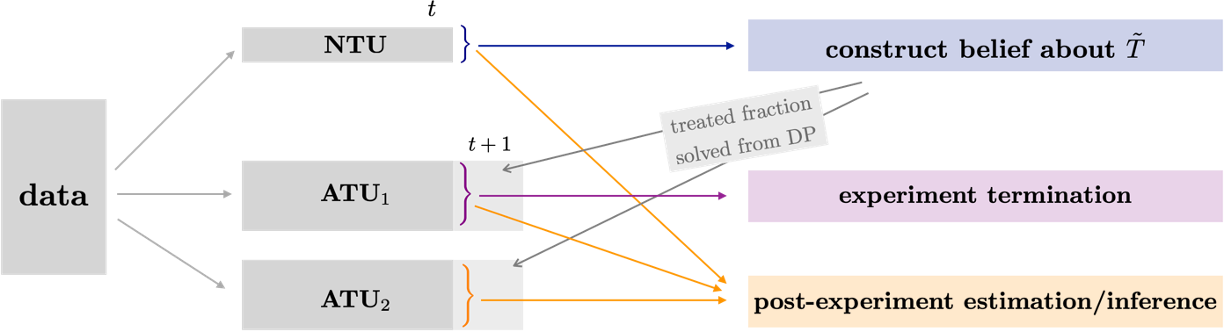
\includegraphics[width=0.8\linewidth]{plots/illustration/pgae.png}
		\caption{\textbf{Illustration of PGAE.}}
		\label{fig:pgae}
	\end{figure}
	
	

Next, we illustrate how PGAE addresses each of the three challenges.

\paragraph{1. Choosing a treatment design.}
{\blue 
In order to update treatment decisions for ATU, we need to construct a belief about experiment stopping time $\tilde{T}$, using NTU. If we would have known $\sigma_\varepsilon^2$, then we would exactly know the minimum stopping time $\tilde{T}$ such that the precision (using $\bm{\omega}_{\mathrm{bm}}$) is bigger than $c$ in \eqref{eqn:experiment-termination-rule}. However, $\sigma_\varepsilon^2$ is unknown in practice, but it is possible to construct \cmtfinal{the belief} distribution of $\sigma_\varepsilon^2$, which will be explained in detail below. Then we can draw samples of $\sigma^2$ from the \cmtfinal{belief} distribution of $\sigma_\varepsilon^2$. For each sampled  $\sigma^2$, we plug it into the precision expression and find the minimum duration that satisfies the stopping rule \eqref{eqn:experiment-termination-rule}.\footnote{Formally, we find $T$ using the following approach. Let $\sigma_0^2$ be a sampled $\sigma^2$ and let $T_0 = \min \left\{t: Nt / \sigma_0^2 \cdot g_\tau(\bm{\omega}, t) \geq c  \right\}$ be the minimum duration such that the precision exceeds threshold $c$. If $T_0 \in \{t+1, t+2, \cdots, T_{\max}\}$, then we set $T$ as $ T_0$; otherwise, if $T_0 > T_{\max}$, then we set $T$ as $T_{\max}$; otherwise, if $T_0 \leq t$, then we set $T$ as $t+1$. } The minimum duration may vary with the sampled $\sigma^2$. By repeatedly sampling $\sigma^2$ and finding the minimum duration, we can obtain an empirical distribution of $\tilde{T}$, denoted as $P_t(\tilde{T})$. See the pseudocode of the helper function \texttt{estimate\_belief()} of PGAE in Section \ref{subsec:pseudo-code} for more details.

Here is our approach to constructing a \cmtfinal{belief} distribution of $\sigma_\varepsilon^2$. We first estimate $\sigma_\varepsilon^2$ from formula \eqref{eqn:second-moment-sigma-estimator} using data of NTU for $t$ periods. Let $\estsigmasq_{\fcs,t}$ be the estimator. Next, we quantify the uncertainty in $\estsigmasq_{\fcs,t}$. From Lemma \ref{lemma:asymptotic-tau-sigma} below, $\estsigmasq_{\fcs,t}$ is consistent and asymptotically normal with
\begin{align}
    \sqrt{|\mathcal{S}_\fcs| \cdot t} \cdot \frac{\estsigmasq_{\fcs,t} - \sigma_\varepsilon^2 }{\hat{\xi}_{\fcs,t}^{\dagger} }   \xrightarrow{d} \mathcal{N}(0,1)\,, \label{eqn:asymptotic-normality-sigmasq}
\end{align}
where $\hat{\xi}_{\fcs,t}^{\dagger} = \big[\estxisq_{\fcs,t} + (\estsigmasq_{\fcs,t})^2/(t-1) \big]^{1/2}$ and $\estxisq_{\fcs,t}$ is estimated from \eqref{eqn:fourth-moment-sigma-estimator} using data of NTU. Let the left-hand side of \eqref{eqn:asymptotic-normality-sigmasq} be $w$. We have $\sigma_\varepsilon^2 = \estsigmasq_{\fcs,t} - w \cdot {\hat{\xi}^\dagger_{\fcs,t}}/{\sqrt{|\mathcal{S}_\fcs| \cdot t}}$, and we repeatedly use this formula with samples of $w$ from $\mathcal{N}(0,1)$ to obtain a \cmtfinal{belief} distribution of $\sigma_\varepsilon^2$. 

We use a dynamic program to solve the treatment decisions for ATU. In this dynamic program, the state variable is the treated fractions up to time $t$, i.e., $\bm{\omega}_{\ad,1:t}$, and the decision variable is the treated fraction for the next period $\omega_{t+1}$.\footnote{{\blue Example 4.3.4 of \cite{bertsekas2012dynamic} also uses a dynamic program to select a threshold for terminating a sequential hypothesis testing problem, but we use a dynamic program to find the optimal design in subsequent time periods.}}  The payoff in intermediate time periods is zero, and conditional on the realization of $\tilde{T}$, the terminal cost is
$- \tilde{T} \cdot \funfrac\left((\bm{\omega}_{\ad,1:t},
\bm{\omega}_{(t+1):\tilde{T}}), \tilde{T}\right)$, which is equivalent to our objective of maximizing precision. 
Here, in the dynamic program, we aim to solve $\omega_{t+1}$ that minimizes the expected terminal cost. The expectation is taken with respect to the random experiment duration $\tilde{T}$, and we use the empirical distribution $P_t(\tilde{T})$ learned at time $t$ when taking the expectation. Specifically, we solve $\omega_t$ by minimizing
% Recalling that $\tilde{T}$ is unknown and information relevant to $\tilde{T}$ is revealed over time, decisions about $\omega_{t+1}$ are based on beliefs about $\tilde{T}$ at time $t$. We solve for $\omega_{t+1}$ by minimizing
%
\[
\+E_{\tilde{T} \sim P_t(\tilde{T})} \left[ - \tilde{T} \cdot \funfrac\left((\bm{\omega}_{\ad,1:t}, \bm{\omega}_{(t+1):\tilde{T}}), \tilde{T}\right) \right]\,,
%
\]
subject to the constraint $\omega_{\ad,t} \leq  \omega_{t+1} \leq  \omega_{t+2} \leq \cdots \leq \omega_{T_{\max}} \leq 1$.\footnote{Only $\omega_{t+1}$ is the decision variable. $\omega_{t+2}, \cdots, \omega_{T_{\max}} $ are not decision variables, whose values can vary with $\tilde{T}$.}
Section \ref{subsec:dp-omega} provides more discussion on this dynamic program, and more details about the dynamic program can be found in the pseudocode of the helper function \texttt{update\_treatment\_design()} of PGAE in Section \ref{subsec:pseudo-code}.

}



\paragraph{2. Implementing the termination rule.} We use the data in $\mathcal{S}_{\ad,1}$ to estimate $\sigma^2_\varepsilon$ via formula \eqref{eqn:second-moment-sigma-estimator}. Let the estimator at time $t$ be $\estsigmasq_{\ad,1,t}$.\footnote{For notation simplicity, we denote the estimator as $\estsigmasq_{\ad,1,t}$, as opposed to $\estsigmasq_{\mathcal{S}_{\ad,1},t}$.}
We then plug $\estsigmasq_{\ad,1,t}$ and $\bm{\omega}_{\mathrm{bm},1:t}$ into the termination rule \eqref{eqn:experiment-termination-rule} to estimate precision and decide whether to terminate the experiment. Note that using $\bm{\omega}_{\mathrm{bm},1:t}$ tends to under-estimate the precision (see Proposition \ref{prop:precision-ordering} in Section \ref{subsec:sequential-additional-results}), so that the experiment termination tends to be conservative. If our experiment terminates, we show in Proposition \ref{prop:precision-guarantee} in Section \ref{subsec:sequential-additional-results} that the true precision exceeds $c$ with a high probability.\footnote{Admittedly, it seems natural to use $\bm{\omega}_{\ad,1:t}$ that may yield a more precise estimation of the precision. We do not pursue this route as it is harder to show that the post-experiment inference of $\tau$ is valid and the corresponding precision is indeed larger than $c$, given the complexity of the current proof.} 



\paragraph{3. Efficient estimation and valid inference for $\tau$.} In PGAE, we estimate 
$\tau$ using all the data of NTU and ATU over $\tilde{T}$ periods. Let the estimator be $\hat{\tau}_{\all,\tilde T}$. We show in Theorem \ref{theorem:asymptotic-page} below that $\hat{\tau}_{\all,\tilde T}$ is efficient and achieves the optimal convergence rate. But we only use $\mathcal{S}_{\ad,2}$ to estimate $\sigma^2_\varepsilon$ via formula \eqref{eqn:second-moment-sigma-estimator}. Let the estimator be $\estsigmasq_{\ad,2,\tilde T}$, which is consistent, and we use $\estsigmasq_{\ad,2,\tilde T}$ to estimate $\var(\hat{\tau})$.
Note that the consistency of $\sigma^2_\varepsilon$ is sufficient for constructing valid confidence intervals for $\tau$. Therefore the efficiency (determined by the sample size) in the estimation of $\sigma^2_\varepsilon$ is less important. The only tradeoff is that the endpoints of confidence intervals are estimated less precisely, with a larger second-order error term.\footnote{The first-order error term comes from the estimation error of $\hat{\tau}_{\all,\tilde T}$} This explains why we use only $\mathcal{S}_{\ad,2}$ to estimate $\sigma^2_\varepsilon$.

In summary, PGAE takes advantage of all the data collected so far, and then jointly optimizes treatment assignments alongside the choice of whether to continue the experiment. The pseudocode for PGAE is shown in Algorithm \ref{algo:page}, with the pseudocode for the helper functions collected in Section \ref{subsec:pseudo-code}. 

\begin{algorithm}[t!]
 \caption{Precision-Guided Adaptive Experiment (PGAE)}  \label{algo:page}
% {\small
  \SetAlgoLined\DontPrintSemicolon
  \SetKwFunction{algo}{algo}\SetKwFunction{proc}{proc}
  \SetKwProg{myalg}{Algorithm}{}{}
  \SetKwFunction{pgae}{pgae}
  \SetKwFunction{Fpart}{partition\_initialize}
  \SetKwFunction{estbelief}{estimate\_belief}
  \SetKwFunction{updatedesign}{update\_treatment\_design}
  \SetKwFunction{estvarprec}{estimate\_var\_prec}
  \myalg{\pgae{$N,T_{\max}, \bm{\omega}_{\mathrm{bm}}, c, p_{\fcs}, m, t_0$}}{
  \nl $Z_{\fcs}$, $Z_{\ad,1}$, $Z_{\ad,2} \leftarrow$ \Fpart{$N, p_{\fcs}, T_{\max}$}\;
  \nl Run the experiment for $t_0$ time periods \;
  \nl $\estsigmasq_{\ad,1,t}, \widehat{\Prec}_{\ad,1,t} \leftarrow$ \estvarprec{$Z_{\ad,1,1:t}, Y_{\ad,1,1:t}, \bm{\omega}_{\mathrm{bm}}, N, n_{\ad}, t$} \;
  \nl \While{$\widehat{\Prec}_{\ad,1,t}  < c$ {\rm and} $t < T_{\max}$}{
  \nl $P_t(\cdot) \leftarrow $ \estbelief{$Z_{\fcs,1:t}, Y_{\fcs,1:t}, N, \bm{\omega}_{\mathrm{bm}}, T_{\max}, t, m, c$}\;
  \nl $Z_{\ad,1,t+1}, Z_{\ad,2,t+1} \leftarrow $ \updatedesign{$Z_{\ad,1,1:t}, Z_{\ad,2,1:t}, \omega_{\ad,1:t}, T_{\max}, t$} \;
  %\nl 
  \nl $t \leftarrow t+1$, and run the experiment for time period $t+1$\;
  \nl $\estsigmasq_{\ad,1,t}, \widehat{\Prec}_{\ad,1,t} \leftarrow$ \estvarprec{$Z_{\ad,1,1:t}, Y_{\ad,1,1:t}, \bm{\omega}_{\mathrm{bm}}, N, n_{\ad}, t$} \;
  
  }
  \nl $\tilde{T} \leftarrow t$, and $\hat{\tau}_{\all,\tilde{T}} \leftarrow$ \within estimator of $\tau$ from both NTU and ATU \;
  \nl $\estsigmasq_{\ad,2,\tilde{T}}, \widehat{\Prec}_{\ad,2,\tilde{T}} \leftarrow$ \estvarprec{$Z_{\ad,2,1:\tilde{T}}, Y_{\ad,2,1:\tilde{T}}, \bm{\omega}_{\mathrm{bm}}, N, n_{\ad}, \tilde{T}$} \;
  \nl \KwRet $\tilde{T}$, $\hat{\tau}_{\all,\tilde{T}}$ and $\estsigmasq_{\ad,2,\tilde{T}}$\;}{}
%   }
\end{algorithm} 

% \tocless
\subsection{Analysis of the Algorithm}\label{subsec:adaptive-theoretical-guarantee}

In this subsection, we present the asymptotic results of the estimated $\tau$ and $\sigma^2_\varepsilon$ in PGAE. These results serve two purposes. The first is to justify our approach in Section \ref{subsec:adaptive-algorithm} to construct a belief about $\sigma^2_\varepsilon$, and specifically to justify \eqref{eqn:asymptotic-normality-sigmasq}. The second is to show that the outputs of PGAE ({\it i.e.}, $\hat{\tau}_{\all,\tilde{T}}$ and $\estsigmasq_{\ad,2,\tilde{T}}$) can be used for valid statistical inference and hypothesis test of treatment effect.


{\blue
To start, we characterize the asymptotic properties of $\hat{\tau}_{\fcs,t}$, $\estsigmasq_{\fcs,t}$ and $\estxisq_{\fcs,t}$, when they are estimated from non-adaptive experimental data, in Lemma \ref{lemma:asymptotic-tau-sigma}. This lemma provides theoretical support for constructing the \cmtfinal{belief} distribution of $\sigma_\varepsilon^2$, and serves as a crucial intermediate step in characterizing asymptotic distributions for the outputs of PGAE. 


\begin{lemma}\label{lemma:asymptotic-tau-sigma}
Suppose Assumptions \ref{ass:treatment-adoption} and \ref{ass:model} hold. Under the specification \eqref{eqn:two-way-direct-model}, suppose $\varepsilon_{is}$ is i.i.d. for any $i$ and $s$ with $\+E[\varepsilon_{is}] = 0$, $\+E[\varepsilon^2_{is}] = \sigma_\varepsilon^2$, $\+E[\varepsilon^3_{is}] = 0$,  and $\+E[(\varepsilon^2_{is} - \sigma^2_\varepsilon)^2] = \xi^2_{\varepsilon}$. $\hat{\tau}_{\fcs,t}$ and $\estsigmasq_{\fcs,t}$ are consistent. As $|\mathcal{S}_{\fcs}| \rightarrow \infty$, for any finite $t$, conditional on $Z_\fcs$, we have 
\[\sqrt{|\mathcal{S}_{\fcs}|} \left(\begin{bmatrix} \hat{\tau}_{\fcs,t} \\ \estsigmasq_{\fcs,t} \end{bmatrix}  - \begin{bmatrix} \tau \\ \sigma^2_\varepsilon  \end{bmatrix}\right)  \stackrel{d}{\longrightarrow } \mathcal{N} \left(\begin{bmatrix} 0 \\ 0 \end{bmatrix}, \begin{bmatrix} \sigma_\varepsilon^2/(t \cdot \funfrac(\bm{\omega}_{\fcs, 1:t}, t)) & 0 \\  0 & \xi_{\varepsilon,t}^{\dagger2}/t \end{bmatrix} \right), \]
where $\xi_{\varepsilon,t}^{\dagger2} = \xi^2_\varepsilon + 2 \big(\sigma_\varepsilon^2\big)^2/(t-1)$. Furthermore, 
$\sqrt{|\mathcal{S}_{\fcs}|} \big(\estxisq_{\fcs,t} - \xi_\varepsilon^2\big) = O_p(1)$.
\end{lemma}

Since both $\estsigmasq_{\fcs,t}$ and $\estxisq_{\fcs,t}$ are consistent, $\estxidaggersq_{\fcs,t} = \estxisq_{\fcs,t} + 2 \big(\estsigmasq_{\fcs,t} \big)^2/(t-1)$ is a consistent estimator of $\xi_\varepsilon^{\dagger2}$. From Slutsky's theorem, the asymptotic distribution in \eqref{eqn:asymptotic-normality-sigmasq} holds.


Interestingly, $\hat{\tau}_{\fcs,t}$ and $\estsigmasq_{\fcs,t}$ are asymptotically independent, even though we use $\hat{\tau}_{\fcs,t}$ in the estimation of $\estsigmasq_{\fcs,t}$. The reason of asymptotic independence is as follows. The estimation error of $\hat{\tau}_{\fcs,t}$ is a weighted average of $\varepsilon_{is}$ over $i$ and $s$. The leading term in the estimation error of $\estsigmasq_{\fcs,t} $ is the sum of a weighted average of $\varepsilon^2_{ju} - \sigma_\varepsilon^2$ over $j$ and $u$ and a weighted average of $\varepsilon_{ju} \varepsilon_{jv} $ over $j,u,v$ with $u \neq v$. Note that $\varepsilon_{is}$ is uncorrelated with both $\varepsilon^2_{ju} - \sigma_\varepsilon^2$ and $\varepsilon_{ju} \varepsilon_{jv} $ for all $i,j,s,u,v$, because $\varepsilon_{is}$ is i.i.d. in $i$ and $s$ and has zero first and third moments. Therefore, the leading terms in the estimation errors of $\hat{\tau}_{\fcs,t}$ and $\estsigmasq_{\fcs,t} $ are uncorrelated. For the non-leading terms, they are at a small order of magnitude and do not contribute to the asymptotic covariance. 
As $\hat{\tau}_{\fcs,t}$ and $\estsigmasq_{\fcs,t}$ are jointly asymptotically normal, the zero asymptotic correlation implies asymptotic independence. In Section \ref{subsec:finite-sample-lemma}, we demonstrate the finite sample properties of Lemma \ref{lemma:asymptotic-tau-sigma} and asymptotic independence between $\hat{\tau}_{\fcs,t}$ and $\estsigmasq_{\fcs,t}$.

\begin{remark}\label{remark:lemma-finite-t}
Lemma \ref{lemma:asymptotic-tau-sigma} holds for any finite $t$. In fact, when $t$ grows to infinity, the problem is simpler, because we can show $\plim_{t\rightarrow \infty} \xi^{\dagger 2}_{\varepsilon,t} = \xi^2_\varepsilon$, and the plug-in estimator of $\xi^2_\varepsilon$ mentioned in formula \eqref{eqn:fourth-moment-sigma-estimator} is consistent. In this section, we focus on the challenging case with a finite $t$, because we want to apply Lemma \ref{lemma:asymptotic-tau-sigma} to the estimates on NTU early in the experiment ({\it i.e.}, $t$ is small).
\end{remark}

}

Next we show that $\hat{\tau}_{\all,\tilde{T}}$ and $\estsigmasq_{\ad,2,\tilde{T}}$ from PGAE can be used for valid post-experiment statistical inference and hypothesis testing for $\tau$. To show this, there are two critical steps: (a) show the asymptotic distribution of $\hat{\tau}_{\all,\tilde{T}}$; (b) show that the asymptotic variance of $\hat{\tau}_{\all,\tilde{T}}$ can be consistently estimated using $\estsigmasq_{\ad,2,\tilde{T}}$.

\begin{theorem}\label{theorem:asymptotic-page}
Suppose Assumptions \ref{ass:treatment-adoption} and \ref{ass:model} hold, $p_{\fcs} \in (0,1)$ is a fixed number as $N$ grows. Under the specification \eqref{eqn:two-way-direct-model}, suppose the assumptions about $\varepsilon_{is}$ in Lemma \ref{lemma:asymptotic-tau-sigma} hold and $\varepsilon_{is}$ is bounded with a symmetric distribution around $0$. $\hat{\tau}_{\all,\tilde{T}}$ and $\estsigmasq_{\ad,2,\tilde{T}}$ are consistent.
As $N \rightarrow \infty$,
        \begin{align}
        \sqrt{N} \cdot \begin{bmatrix}
    \big(\tilde{T}\funfrac(\bm{\omega}_{\all,1:\tilde{T}},\tilde{T})/\sigma_\varepsilon^2\big)^{1/2} \cdot \left( \hat{\tau}_{\all,\tilde{T}} - \tau\right) \vspace{0.3cm}  \\ \big(\tilde{T} p_{\ad,2}/\xi^{\dagger 2}_{\varepsilon,\tilde{T}} \big)^{1/2} \cdot \big(\estsigmasq_{\ad,2,\tilde{T}} - \sigma_\varepsilon^2 \big)
        \end{bmatrix}
        \stackrel{d}{\longrightarrow } \mathcal{N} \left(\bm{0}, I_2 \right) \label{eqn:cond-normal}\, .
    \end{align}
    \end{theorem}
{ 

\cmtrx{$\hat{\tau}_{\all,\tilde{T}}$ is consistent for $\tau$ with the optimal convergence rate $\sqrt{N}$. This result is not obvious because $\mathcal{S}_{\fcs}$, $\mathcal{S}_{\ad,1}$ and $\mathcal{S}_{\ad,2}$ are all used to estimate $\tau$, which could potentially lead to two sources of bias in the estimation of $\tau$. The first is that $\hat{\tau}_{\all,\tilde{T}}$ depends on adaptive treatment designs, and the choice of adaptive designs depend on  $\estsigmasq_{\fcs,t}$ and $\estxisq_{\fcs,t}$, and therefore on $\varepsilon_{is}$ for $i \in \mathcal{S}_{\fcs}$. The second is that $\hat{\tau}_{\all,\tilde{T}}$ depends on termination time $\tilde{T}$, where $\tilde{T}$ depends on $\estsigmasq_{\ad,1,t}$ and therefore on $\varepsilon_{is}$ for $i \in \mathcal{S}_{\ad,1}$. Both sources may lead to the violation of the commonly made exogeneity assumption  to show consistency ({\it i.e.}, asymptotic conditional mean of $\varepsilon_{it}$ is zero). With a careful analysis in Lemma \ref{lemma:conditional-mean-variance}, we show this is not the case, and the asymptotic conditional mean is still zero. This is mainly because $\estsigmasq_{\fcs,t}$, $\estxisq_{\fcs,t}$ and $\estsigmasq_{\ad,1,t}$ are all even moments of $\varepsilon_{is}$. With a symmetric distribution of $\varepsilon_{is}$ around $0$, conditioning on the even moments does not change the mean of $\varepsilon_{is}$.}

\cmtrx{
The adaptivity of the design, with the termination time depending on early values of the outcomes, comes at no cost in the estimation of $\tau$ in the following sense. Suppose we run an adaptive experiment, with a distribution of termination times. Now suppose we compare this to a series of non-adaptive experiments with the same distribution of termination times. This series of non-adaptive experiments is not actually feasible, because it depends on values we do not know {\it ex ante}. Nevertheless, this series of experiments does not do better than our proposed adaptive experiment, in the sense that the average of the variances is the same as that for our proposed adaptive experiment. This result is surprising as the adaptive nature in choosing treatment designs and in experiment termination does not affect the estimation efficiency of $\hat{\tau}_{\all,\tilde{T}}$. In Section \ref{subsec:finite-sample-pgae}, we empirically show that the results of Theorem \ref{theorem:asymptotic-page} are valid for a moderate $N$.}

Moreover, as our adaptive treatment decisions seek to maximize $\funfrac(\cdot)$, we expect $\funfrac(\bm{\omega}_{\all,1:\tilde{T}},\tilde{T}) > \funfrac(\bm{\omega}_{\mathrm{bm},1:\tilde{T}},\tilde{T})$ so that $\tau$ can be estimated more efficiently than the benchmark design ({\it i.e.}, $\Prec(\hat{\tau}_{\all,\tilde{T}}) > ({N\tilde{T}}/{\sigma^2_\varepsilon}) \cdot \funfrac(\bm{\omega}_{\mathrm{bm},1:\tilde{T}},\tilde{T})$). This is shown in Proposition \ref{prop:precision-ordering} in Section \ref{subsec:sequential-additional-results} for a large $N$, and is empirically demonstrated in Section \ref{subsec:empirical-sequential} for a moderate $N$.
}


\subsection{Extension to Carryover Model with Covariates}\label{subsec:sequential-carryover}

PGAE and Theorem \ref{theorem:asymptotic-page} can be easily extended to the specification with $\ell > 0$ and with $\*X_i$. We can continue using the \within estimator for $\tau_0, \cdots, \tau_\ell$ by regressing $\dot{Y}_{it}$ on $\dot{z}_{it}, \cdots, \dot{z}_{i,t-\ell}, \dot{\*X}_i$. For the experiment termination rule, we could generalize \eqref{eqn:experiment-termination-rule} to $\tr \big(\mathrm{Prec}(\hat{\bm{\tau}})  \big) \geq c$ or other criteria based on the objectives discussed in Section \ref{subsec:objective}. From Lemma \ref{lemma:simplify-obj} in Section \ref{subsec:separate-quadratic}, the only unknown parameter in the termination rule is $\sigma_\varepsilon^2$. Furthermore, we can partition units into strata based on $\*X_i$. For each stratum, we can then continue using PGAE to construct an empirical distribution about $\tilde{T}$, make adaptive treatment decisions, and sequentially decide whether to terminate the experiment. We can use a similar proof to show that results in Section \ref{subsec:adaptive-theoretical-guarantee} continue to hold with $\hat\tau$ replaced by $\hat\tau_0, \cdots, \hat\tau_\ell$ and $g_{\tau}(\bm{\omega},\tilde{T}) $ replaced by a matrix depending on $\bm{\omega}$ and $\tilde{T}$ (see Lemma \ref{lemma:simplify-obj} for its definition). 


{\blue If the specification has $\*u_i$, there are multiple approaches to proceed. First, as a simple solution, we can ignore $\*u_i$ and run PGAE as the case without $\*u_i$. This approach can be shown to be valid under suitable assumptions.\footnote{For example, the suitable assumptions can be $\*u_i$ is mean zero and i.i.d. in $i$, and $\*v_s$ is i.i.d. in $s$.} We can further improve the precision of $\hat{\tau}_{\all,\tilde{T}}$ by re-estimating $\tau$ using GLS post-experiment.

Second, as a more efficient solution, if we have historical data, then we can use it to estimate $\*u_i$, partition units into strata, and run PGAE on each stratum. With abundant historical data, we can precisely estimate $\sigma_\varepsilon^2$, and therefore the minimum duration to achieve a certain precision threshold. For this case, we do not need an adaptive experiment and can instead run the non-adaptive experiment with the estimated minimum duration.}